\chapter{Attaque SSLstrip}

\label{sec:sslstrip}

\begin{figure}[H]
  \caption{Attaque SSLstrip (diagramme Dia)}
  \fbox{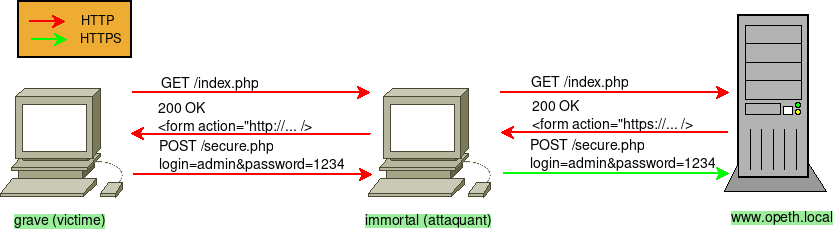
\includegraphics[width=\textwidth]{../medias/sslstrip/attack.png}}
\end{figure}

Le But de l'attaque est de rediriger tout trafic https vers du http sans que la victime s'en aperçoive.

Il faut transformer tous les liens https en http et il faudra garder en mémoire tous les changement effectués.

Pour cela, il faut d'abord mettre en place le Man in the Middle.

Il faut donc mettre en place un ARP poisonning qui va se charger de faire croire à la victime que notre addresse MAC est celle du routeur.

L'attaque doit se passer soit lors des redirections 302, soit quand l'utilisateur clique sur un lien HTTPS.

Les actions à mettre en place :
1. Regarder le trafic HTTP
2. Changer les liens https par des https et garder en mémoire les actions
3. Lorsque qu'on voit une requête HTTP pour une URL que l'on a supprimé, il faut envoyer au serveur du HTTPS
4. Conserver une carte des liens relatifs, CSS, JavaScript
5. Pour essayer de conserver le même aspect visuel, on doit faire de même pour les favicon en renvoyant la favicon de notre choix.
6. A éliminer des en-têtes de requêtes, les encodages, les cookies et les pages en cache.
7. Lors des requêtes POST envoyées par SSL, avec login et password, il faut faire expirer les cookies pour que l'utilisateur renvoie une requête sans cookies

------

L'attaque sslstrip a été présentée pour la première fois en 2009 par l'américain Moxie Marlinspike à la conférence en sécurité Blackhat. C'est une attaque très simple qui va permettre à un attaquant de pouvoir récupérer des informations confidentielles telles qu'un mot de passe ou un cookie de session. Cependant, l'attaque n'est plus vraiment d'actualité, nous reviendrons là dessus à la fin.

Pour que l'attaquant puisse utiliser sslstrip, il doit pouvoir se placer en homme du milieu entre le client et le serveur. C'est à dire qu'il doit être capable d'intercepter le trafic entre ces deux derniers, et pouvoir le modifier à sa guise. Bien sûr, l'attaquant n'a aucun intérêt à substituer une requête du client pour envoyer n'importe quoi à la place, car le serveur ne comprendra pas la requête et fermera la connexion TCP. Il va donc falloir être astucieux dans la manière dont on agit.

Pour pouvoir se placer en MITM, il y a plusieurs façons de procéder. Une des façons les plus simples consiste à se placer dans le réseau privé dans la victime, et de faire un ARP spoofing. L'idée étant de faire croire au routeur qu'il parle à la victime, et vice versa, en falsifiant leur table arp respective (cette table donnant la correspondance entre adresse mac et adresse ip). L'attaquant va ainsi pouvoir lire tout le traffic qui circule entre la victime et le routeur (donc entre la victime et le serveur).

*** Faut-il expliquer plus en détail l'ARP ? ***

Une fois placée en homme du milieu, l'attaquant peut donc voir le traffic envoyé par la victime vers le serveur. Bien sûr, si ce traffic est chiffré, par exemple avec le protocol SSL/TLS en https, alors l'attaquant ne pourra rien en tirer, à moins de trouver une faille dans le chiffrement utilisé. Ici, on ne va pas essayer de casser TLS, mais plus de profiter du fait que toutes les requêtes envoyées par le client ne sont pas chiffrées (c'est de moins en moins vrai de nos jours).

Ainsi, si la requête du client est une simple requête http, l'attaquant va pouvoir lire ce qu'il envoie, et mieux encore, il va également voir la réponse du serveur.

On sait donc maintenant que notre attaquant peut, si la requête n'est pas chiffrée, lire l'échange effectué entre le client et le serveur, et même le modifier un peu si la requête reste valide et compréhensible par le serveur. Mais, qu'est-ce qu'on va bien pouvoir modifier pour obtenir des informations intéressantes ?

Pour répondre à cette question, il faut savoir que toutes les pages sensibles d'un site internet (qui demandent une connexion avec identifiant/mot de passe), ne sont accessibles que par une requête sécurisée en https (ou alors le site est vraiment peu précautionneux). Lorsqu'un page html contient des liens vers des pages sécurisées, ces liens sont donc en https, pour indiquer au client qu'un chiffrement va être nécessaire à la connexion d'une page en particulier.

\begin{figure}[H]
  \caption{Exemple d'une page html avec un lien sécurité https}
  \fbox{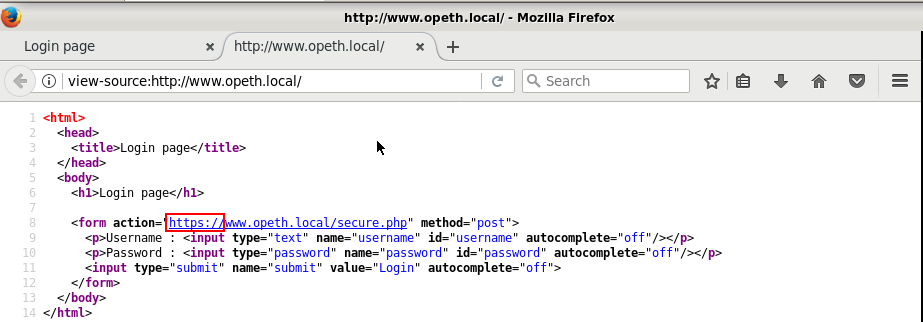
\includegraphics[width=\textwidth]{../medias/sslstrip/screen2.png}}
\end{figure}

L'idée de l'attaque, va donc être de forcer le client à se connecter en http, et non en https, sur la page sensible. Pour cela, rien de plus simple : lorsque le serveur va envoyer une page html contenant des liens https, l'attaquant va simplement intercepter la page html, retirer le 's' de chacun de ces liens, et envoyer la page au client. Lorsque ce dernier voudra se connecter sur ces liens, il le fera donc en http et non en https comme il l'aurait fallu. L'attaquant va donc pouvoir lire tout le traffic de cette requête http, contenant par exemple un mot de passe si la page sécurisée était un formulaire de connexion.

\begin{figure}[H]
  \caption{La même page html, où l'attaquant a strip un 's'}
  \fbox{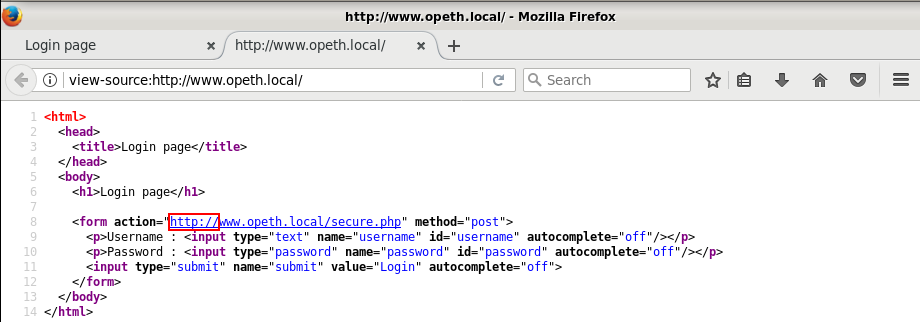
\includegraphics[width=\textwidth]{../medias/sslstrip/screen5.png}}
\end{figure}

*** recoper plus ou moins la description de l'attaque du README ? ***

Cependant, l'attaque n'est plus vraiment d'actualité car les sites internet modernes (ou plutôt, ceux qui pensent à la sécurité de leurs utilisateurs), utilisent https sur toutes les pages de leur site web, ce qui empêche l'attaquant d'intercepter ne serait-ce qu'une requête http, et de la modifier. De plus, une autre protection, nommée HSTS, permet au serveur d'indiquer à un client de toujours se connecter en https sur certaines pages. Ainsi, si un attaquant parvient à intercepter une requête http, et à remplacer les liens https vers des liens http dans le code html, le navigateur du client emettra une exception, car il aura gardé en mémoire qu'il doit se connecter en https sur telle page spécifique. Néanmoins il existe des moyens de contourner cet ajout, nous en parlerons dans la prochaine attaque.
